\documentclass{article}

\usepackage[T1]{fontenc}
\usepackage[utf8]{inputenc}

\usepackage{amsmath, amssymb, amsfonts}
\usepackage[margin=3cm]{geometry}
\usepackage{listings}
\usepackage{graphicx}

\begin{document}
\section*{Exercise 1}
    We have
    \[
        \phi''(x) = A.
    \]
    If \(A\) is positive semidefinite, we can apply Theorem 2.9 (a) and conclude that \(\phi\) is convex.

    Now we have to show the equivalences. 
    \begin{itemize}
        \item[(a) $\implies$ (b)] If there is a global minimizer, $\phi$ has to be bounded below by definition.
        \item[(b) $\implies$ (c)] Assume that there is an eigenvector $v$ of $A$ with eigenvalue $0$ s.t. $b^\top v \neq 0$.
        Let $-C$ be a lower bound for $\phi$. Then choose 
        \[
            \lambda := \frac{C + c + 1}{b^\top v}.
        \]
        We obtain a contradiction,
        \[
            \phi(\lambda \cdot v) = (\lambda v)\top A (\lambda v) - b^\top v + c = 0 - \frac{C + c + 1}{b^\top v} \cdot (b^\top v) + c = - C - 1.
        \]
        Therefore, $b$ is in the orthogonal complement of the eigenspace to the eigenvalue 0. In particular, we find $\alpha_i$ s.t.
        \[
            b = \sum_i \alpha_i v_i,  
        \]
        where $v_i$ is an eigenvector of $A$ with eigenvalue $\lambda_i \neq 0$.
        With
        \[
            x = \sum_i \frac{\alpha_i}{\lambda_i} v_i \implies Ax = \sum_i \alpha_i v_i = b
        \]
        we have found a solution for $Ax = b$.
        \item[(c) $\implies$ (a)] Let $x$ be a solution for $Ax = b$. Then, $\nabla \phi(x) = Ax - b = 0$ and as $\phi$ is convex, the desired implication follows from Sheet 1, Ex. 4.
    \end{itemize}
    Let $v$ be an eigenvector of $A$ with eigenvector $\lambda < 0$. Then, using the Cauchy-Schwarz-inequality and the triangle inequality, we obtain
    \[
        x^\top A x - b^\top x + c \leq \lambda \lVert x\rVert + \lVert b\rVert\lVert x\rVert + c.
    \]
    This is a quadratic polynomial with negative leading coefficient, i.e. it is not bounded below.
\section*{Exercise 2}
\begin{enumerate}
    \item[(i)]
    \begin{itemize}
        \item["$\supseteq$"] Let $d \in \operatorname{RHS}$. By definition,
        \[
            (-\nabla f(x))^\top \cdot d > 0 
        \]
        We apply $\operatorname*{BFGS}$ for $g = (-\nabla f(x))$ and $d = d$ to the identity matrix. Thus, $M^{-1} \cdot (-\nabla f(x)) = d$ and $d \in \operatorname*{LHS}$.
        \item["$\subseteq$"] Take $-M^{-1} \cdot \nabla f(x)\in \operatorname*{LHS}$ for any s.p.d. matrix $M$. Then,
        \[
            f'(x) \cdot (-M^{-1}) \cdot \nabla f(x) = - \lVert\nabla f(x)\rVert^2_{M^{-1}} < 0.
        \]
        Therefore, \(-M^{-1} \cdot \nabla f(x) \in \operatorname{RHS}\).
    \end{itemize}
\item[(ii)] \lstinputlisting[language=python,breaklines=true]{2_ii.py}
\begin{figure}[ht]
    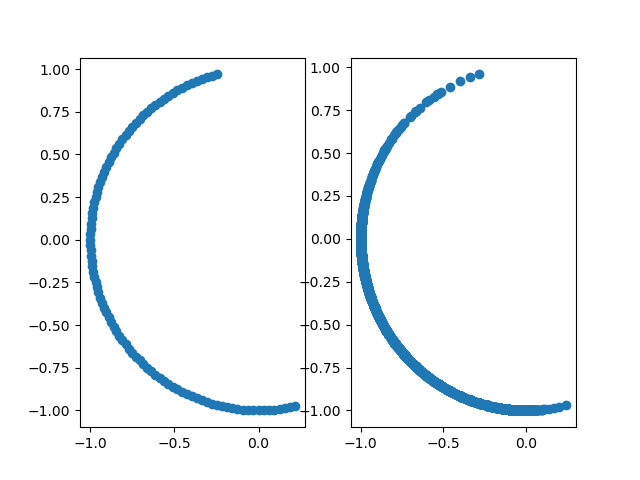
\includegraphics[width=\textwidth]{2_ii_2d_plot.png}
    \caption{Here we show first the right set and then our approximation for the left set.}
\end{figure}
\end{enumerate}

\section*{Exercise 3}
    As shown in the lecture, we have the generalized spectral decomposition
    \[ A = MV\Lambda V^\top M, \]
    s.t. $V^\top M V = \operatorname*{Id}$. This implies $VV^\top = M^{-1}$. 
    and $M^{-1}V^{-\top} = V$.
    Therefore we can compute
    \[
        A^{-1}  = M^{-1} V^{-\top} \Lambda^{-1} V^{-1} M^{-1}
                = V \Lambda^{-1} V^\top
    \] 
    Thereby we get
    \begin{align*}
        \lVert x^{(k)} - x^*\rVert _A^2 &= \lVert A^{-1}r^{(k)}\rVert _A^2\\
        &= r^{(k), \top} A^{-1} A A^{-1} r^{(k)}\\
        &= r^{(k)} V \Lambda^{-1} V^\top r^{(k)}
        \intertext{Using that $\Lambda$ is the diagonal matric of eigenvectors, we obtain}
        \frac{1}{\beta} r^{(k), \top} V \Lambda^{-1} V^\top r^{(k)} &\leq r^{(k), \top} V \Lambda^{-1} V^\top r^{(k)} \leq \frac{1}{\alpha} r^{(k),\top} V V^\top r^{(k)}
    \end{align*}
    Analogously, we compute
    \[
        A^{-1}MA^{-1}   = V \Lambda V^\top M V \Lambda V^\top
                        = V \Lambda^{-2} V^\top
    \] 
    and get
    \begin{align*}
        \lVert x^{(k)} - x^*\rVert _M^2 &= \lVert A^{-1}r^{(k)}\rVert _M^2\\
        &= r^{(k), \top} A^{-1} M A^{-1} r^{(k)}\\
        &= r^{(k), \top} V \Lambda^{-2} V^\top r^{(k)}
        \intertext{Using that $\Lambda$ is the diagonal matric of eigenvectors, we obtain}
        \frac{1}{\beta} r^{(k), \top} V \Lambda^{-2} V^\top r^{(k)} &\leq r^{(k), \top} V \Lambda^{-2} V^\top r^{(k)} \leq \frac{1}{\alpha^2} r^{(k),\top} V V^\top r^{(k)}
    \end{align*}
    Finally, we have
    \[
        \lVert r^{(k)} \rVert _{M^{-1}}^2 =  r^{(k), \top}M^{-1}r^{(k)} = r^{(k), \top}VV^\top r^{(k)}
    \]
    After taking square roots, we can directly see that both cases of bracket (2) hold.
    In order to prove bracket (1), we need to replace $(k)$ by $(0)$ so that we get the following inequality
    \[
        \frac{1}{\sqrt{\beta}} \sqrt{r^{(0), \top} V \Lambda^{-1} V^\top r^{(0)}} \leq \sqrt{r^{(0), \top} V \Lambda^{-1} V^\top r^{(0)}}. \hspace*{3cm}(*)
    \]
    Multiplying with $\sqrt{\beta}$, we can combine it with one of the above inequalities to obtain the desired result:
    First, we find an upper bound for $\lVert x^(k) - x^*\rVert _A$ by $\frac{1}{\sqrt{\alpha}} \lVert r^{(k)}\rVert _{M^{-1}}$.
    Then, we use the given inequality and finally apply $(*)$.
    The second case in bracket (1) works analogously.
    Brackets (3) and (4) can be shown by the exact same procedure as bracket (1).
\section*{Exercise 4}
\lstinputlisting[language=python,breaklines=true]{4.py}
\begin{figure}
    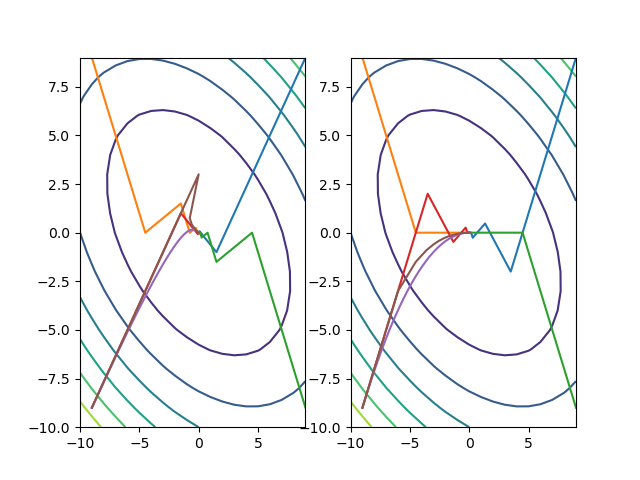
\includegraphics[width=\textwidth]{example.png}
    \caption{We clearly see how different preconditioners produce a different convergence behavior}
\end{figure}
\end{document}